% \iffalse
\let\negmedspace\undefined
\let\negthickspace\undefined
\documentclass[journal,12pt,twocolumn]{IEEEtran}
\usepackage{cite}
\usepackage{amsmath,amssymb,amsfonts,amsthm}
\usepackage{algorithmic}
\usepackage{graphicx}
\usepackage{textcomp}
\usepackage{xcolor}
\usepackage{txfonts}
\usepackage{listings}
\usepackage{enumitem}
\usepackage{mathtools}
\usepackage{gensymb}
\usepackage{comment}
\usepackage[breaklinks=true]{hyperref}
\usepackage{tkz-euclide}
\usepackage{listings}
\usepackage{gvv}
\def\inputGnumericTable{}
\usepackage[latin1]{inputenc}
\usepackage{color}
\usepackage{array}
\usepackage{longtable}
\usepackage{calc}
\usepackage{multirow}
\usepackage{hhline}
\usepackage{ifthen}
\usepackage{lscape}

\newtheorem{theorem}{Theorem}[section]
\newtheorem{problem}{Problem}
\newtheorem{proposition}{Proposition}[section]
\newtheorem{lemma}{Lemma}[section]
\newtheorem{corollary}[theorem]{Corollary}
\newtheorem{example}{Example}[section]
\newtheorem{definition}[problem]{Definition}
\newcommand{\BEQA}{\begin{eqnarray}}
\newcommand{\EEQA}{\end{eqnarray}}
\newcommand{\define}{\stackrel{\triangle}{=}}
\theoremstyle{remark}
\newtheorem{rem}{Remark}
\begin{document}

\bibliographystyle{IEEEtran}
\vspace{3cm}

\title{GATE -BM 16}
\author{EE23BTECH11057 - Shakunaveti Sai Sri Ram Varun$^{}$% &lt;-this % stops a space
}
\maketitle
\newpage
\bigskip
\vspace{2cm}
\textbf{Question: }
A buoy of virtual mass 30 kg oscillates in a fluid medium as a single degree of
freedom system. If the total damping in the system is set as 188.5 N-s/m, such
that the oscillation just ceases to occur, then the natural period of the system is
\rule{1cm}{0.15mm} s (round off to one decimal place)
\hfill(GATE MN 2023 question 63)\\

\textbf{Solution}:\\
\begin{table}[h!] 
\centering
\begin{tabular}{|c|c|c|}
    \hline
    \textbf{Parameter} & \textbf{Description} & \textbf{Value} \\
    \hline
    $X\brak{s}$ & position in laplace domain & $ X\brak{s}$ \\
    \hline
    $\Theta\brak{s}$ & angle rotated in laplace domain & $ \Theta\brak{s}$ \\
    \hline
    $x\brak{t}$ & position of mass w.r.t time & $x\brak{t}$ \\
    \hline
    $\theta\brak{t}$ & angle rotated by mass w.r.t time &$ \theta\brak{t}$\\
    \hline
    $\alpha\brak{t}$ & angular acceleration of mass w.r.t time & $\alpha\brak{t}$ \\
    \hline
    $k$ & spring constant & $ k$\\
    \hline
    $m$ & mass of the block & $ m$\\
    \hline
    $L$ & length of the mass & $ L$\\
    \hline
    $\omega_o$ & initial angular velocity of mass & $ \omega_o$ \\
    \hline
    $v\brak{0}$ & initial velocity of mass& $ v\brak{0}$ \\
    \hline
    
\end{tabular}






\caption{input values}
\label{tab: Table mn63}
\end{table}

The differential equation of the system is:
\begin{align}
m\frac{d^2x\brak{t}}{dt^2} + \lambda \frac{dx\brak{t}}{dt} + m\omega_0^2 x\brak{t} &= 0
\end{align}
Taking laplace transform:
\begin{align}
ms^2X\brak{s} + \lambda s X\brak{s} + m\omega_o^2 X\brak{s}&=0\\
\implies ms^2 + s\lambda + m\omega_o^2 &=0\\
\therefore s = \frac{-\lambda \pm \sqrt{\lambda^2 - 4 m^2 \omega_o^2}}{2m}
\end{align}
where $ \sqrt{\lambda^2 - 4 m^2 \omega_o^2}$ is $ \omega_d$.\\
From \tabref{tab: Table mn63},
\begin{align}
\omega_d &=0\\
\implies \lambda &= 2\omega_o m\\
\implies \omega_o &\approx \pi\\
 T_i &= \frac{2\pi}{\omega_o}\\
 \therefore t_i = 2\text{ seconds}
\end{align}
To find x\brak{t}, we assume the initial amplitude of oscillations to be 1 meter and it is situated at extreme position.
\begin{align}
s^2X\brak{s} + \lambda s X\brak{s} + \omega_o^2 X\brak{s}&=sx\brak{0}+x\brak{0}\\
\implies X\brak{s}&=\frac{1+s}{s^2 + s\lambda + \omega_o^2}
\end{align}
substituting values from \tabref{tab: Table mn63} and $\omega_o$,
\begin{align}
X\brak{s} &= \frac{1+s}{\brak{s+\pi}^2}
\end{align}
\vspace{3cm}

Taking inverse laplace transform by method of partial fractions,
\begin{align}
X\brak{s} &= \frac{1}{s+\pi} + \frac{1-\pi}{\brak{s+\pi}^2}\\
\therefore x\brak{t} &= \brak{1+ \brak{1-\pi}t}e^{-\pi}
\end{align}
\begin{figure}[h!]
    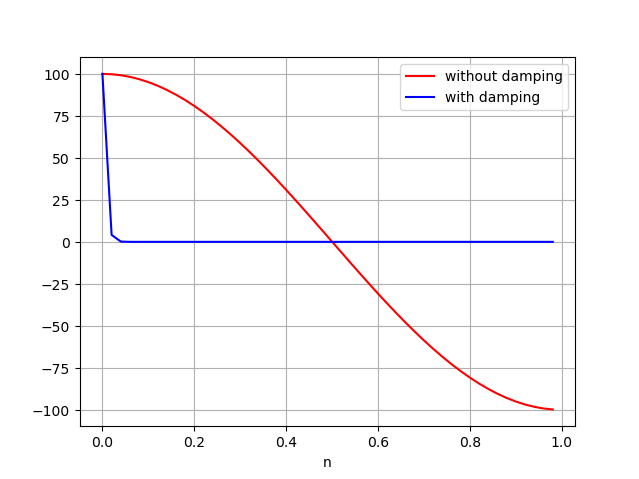
\includegraphics[width = \columnwidth]{figs/Figure_1.png}
    \caption{$ x\brak{t}$ with and with out damping }
    \centering
    \label{fig: nm_63_fig_3}
\end{figure}
\end{document}

